\section{Viscous: Protocol Descriptions}
To overcome the limitations of existing transport layer protocols as discussed in the previous section, we propose a new end-to-end protocol called Viscous. It is a connection oriented multi-path multi-flow protocol which is not coupled with the network stack, and work as a wrapper or a middleware in between the users' application and the transport layer of the network protocol stack. The basic design philosophies for Viscous are as follows. 
\begin{enumerate}
	\item To mitigate the signaling overhead associated with connection establishment, Viscous multiplexes multiple flows over a single Viscous connection. This reduces the connection setup time for short-lived flows. 
	\item Viscous does not maintain a separate and independent congestion control for every application flows. Rather, it maintains a single congestion control mechanism for a Viscous connection which is a multiplex of multiple flows. Further, the congestion control is path specific, that is, congestion is monitored at every path from a source to a destination, where a Viscous sub-flow is initiated.  
	\item To handle HOL blocking problem, Viscous decouples congestion control from the flow control. The Viscous flow control manages the data generation rate from the applications, whereas the congestion control maintains the rate of traffic ingestion into the paths based on congestion feedback. However, to avoid buffer overflow, a feedback is forwarded from the congestion control to the flow control module, whenever necessary.
	\item Viscous follows a modular architecture for ease development of applications. Any Viscous module can be tuned independently to make it suitable for a specific requirement. This way, application layer quality of service (QoS) can be provided with the help of Viscous. 
	\item Viscous works on top of UDP, similar to Goggle's QUIC; therefore it mitigates the transport layer protocol overhead which is associated with TCP. 
	\item Viscous supports different types of mobility without breaking an existing connection. With the help of a unique client and server specific identifier which is shared during the initial connection establishment, Viscous can continue with the existing connection, even if the server or the client changes its IP address.   
\end{enumerate}

\begin{figure}[!t]
	\centering
	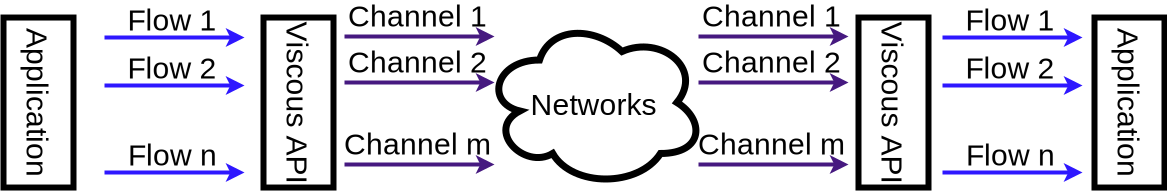
\includegraphics[width=\linewidth]{img/sys-io}
	\caption{Flow-Channel architecture in the Viscous protocol. Application sends and receives data through the flows. Internally, Viscous sends and receives data using multiple channels over multiple paths.}
	\label{fig:sys-io}
\end{figure}

\subsection{Key Concepts Behind the Design of Viscous}
Viscous follows a layered architecture with two different layers, as shown in Fig.~\ref{fig:sys-io}. There are two key concepts behind the design, development, and implementation of Viscous to support ubiquitous transport of data over any Internet devices -- \textit{channel} and \textit{flow}. 

\subsubsection{Channel}
Viscous channels are individual connections between two devices over multiple paths. Paths are defined by compatible source and destination IP pair. There is one single channel for each path. To avoid connection time path imbalance like MPTCP, as we observe in Fig.~\ref{fig:timeSentOverPath}, we initiate all the channels simultaneously after connection establishment and before any flows can start. Connections are established specific to a destination host whenever an application from a source host requests for a connection. This connection is shared with other applications which intend to send data to the same destination host. This way, flows are multiplexed specific to a destination host.

Here connection means Viscous connection. Channels are similar to individual TCP connections or sub-flows in the MPTCP. Each channel has dedicated buffer to provide reliable packet transmission and have congestion control algorithm not to overflow the network. Channels are identified by four tuple of source IP, source interface id, destination IP and destination interface id. Interface id are unique id for each network interface available in a device. All channels are treated as regular, and every channel can participate in transmitting packets from any flows. However, based on other properties like RTT and goodput, one channel can carry more packets than others.


In Viscous, individual application flows do not require separate connection establishment as the connection has already been established between the source and the destination during Viscous connection initiation. Viscous handles congestion control for every individual paths between a source and a destination. Therefore, flow specific congestion control is not required for Viscous, and Viscous maintains path specific congestion control. This way Viscous avoids slow start for every individual flows that share the complete path from the source to the destination. Consequently, channels are persistent in Viscous, and they do not die out after the completion of a flow. As mentioned, a channel can carries data from multiple flows simultaneously by multiplexing them. If one or both the devices are multi-homed, multiple channels can be established that share the traffic load and therefore, achieve better performance.

\subsubsection{Flow} 
Flows in Viscous are responsible for data communication while maintaining the flow-control between a source and a destination. An application can transmit data over multiple flows simultaneously. The user application sends data as byte-streams to the flow, and it also receives data in the form of byte-streams from a flow. Flow is responsible for packetizing the byte-stream and sending the packets to the lower layer of Viscous. Viscous puts packets from flows to channels, and the channels take care of the congestion control. This way, we decouple congestion control from flow control in Viscous design. 

This channel-flow decoupled architecture gives Viscous the power of utilizing multiple paths even for short-lived flows. Flows do not have to suffer from slow start or connection establishment overhead. The connection establishment is a separate event from channel management, and all the channels between a source and a destination start simultaneously. This removes the problem of path selection as we observe in MPTCP.  Further, channel gives an option to support mobility. If one or both the devices change its network address, the associated channel cannot communicate anymore. Viscous can discard the affected channels and initiate new channels using the new network address without any interruption in Viscous connection (application flows). 


\subsubsection{Channel Scheduler}
The Viscous channel scheduler schedules packets from application flows to one of the channels. The channel scheduler have two basic part. i) Load balancer ii) scheduler. The load balancer part is responsible for collecting packets from flows. It is important because it can prioritize one or more flows as per requirement. Although we haven't implemented any priority in our implementation, but we have provision to do it. On the other hand, scheduler is the most important module of our protocol. It decides the way to use multiple channels when different channels have different properties. An ideal scheduler would schedule packet in such a way so that packets arrived on other in ordered fashion. However, to do it, Viscous need to predict future channel condition and application condition which is not feasible. So, we settled with feasible scheduling policies.

First and straightforward way to schedule a packet is to allocate packets to channels in round robin way. In this scheduling policy, scheduler will try to schedule every next packet to next channel if the next channel have space in its $cwnd$, otherwise move next to next channel until scheduler exhaust all the channels. It is easy to deploy, but it is extremely in efficient as we may schedule more packets than required to a slow channel if its $cwnd$ is large.

So, to develop a better scheduler, we developed an acknowledgment(ACK) driven scheduling scheme. Here scheduler schedules a packet to a channel when it receives ACKs and free some space in its $cwnd$. This provides a \textbf{self-clocking behaviour} to the channel scheduler. However, this scheduling works when scheduler buffer always have some packet to send to channels. It is not practical when application trying to send multiple short data. There are phased in between two transmission, when scheduler buffer starves. In those situations, scheduler schedules packets only a channel, and don't put packets to other channels.

Finally, we land to the default MPTCP scheduler. Here, we try to schedule packet packet to a channel with lowest $RTT$ if its $cwnd$ have space for a packet, otherwise move to the channel with second highest $RTT$ and so on. 


\subsection{Connection Establishment: Channels and Flows Creation}

Viscous is a connection oriented protocol. So it uses the client-server architecture for creating and maintaining the connections. A Viscous server waits for a new connection from a Viscous client. 
For each client connection, the server maintains separate sets of channels and other associated modules. In Viscous, communication is possible only after association of the flows to the connections.  

%\begin{figure}[!t]
%	\centering
%	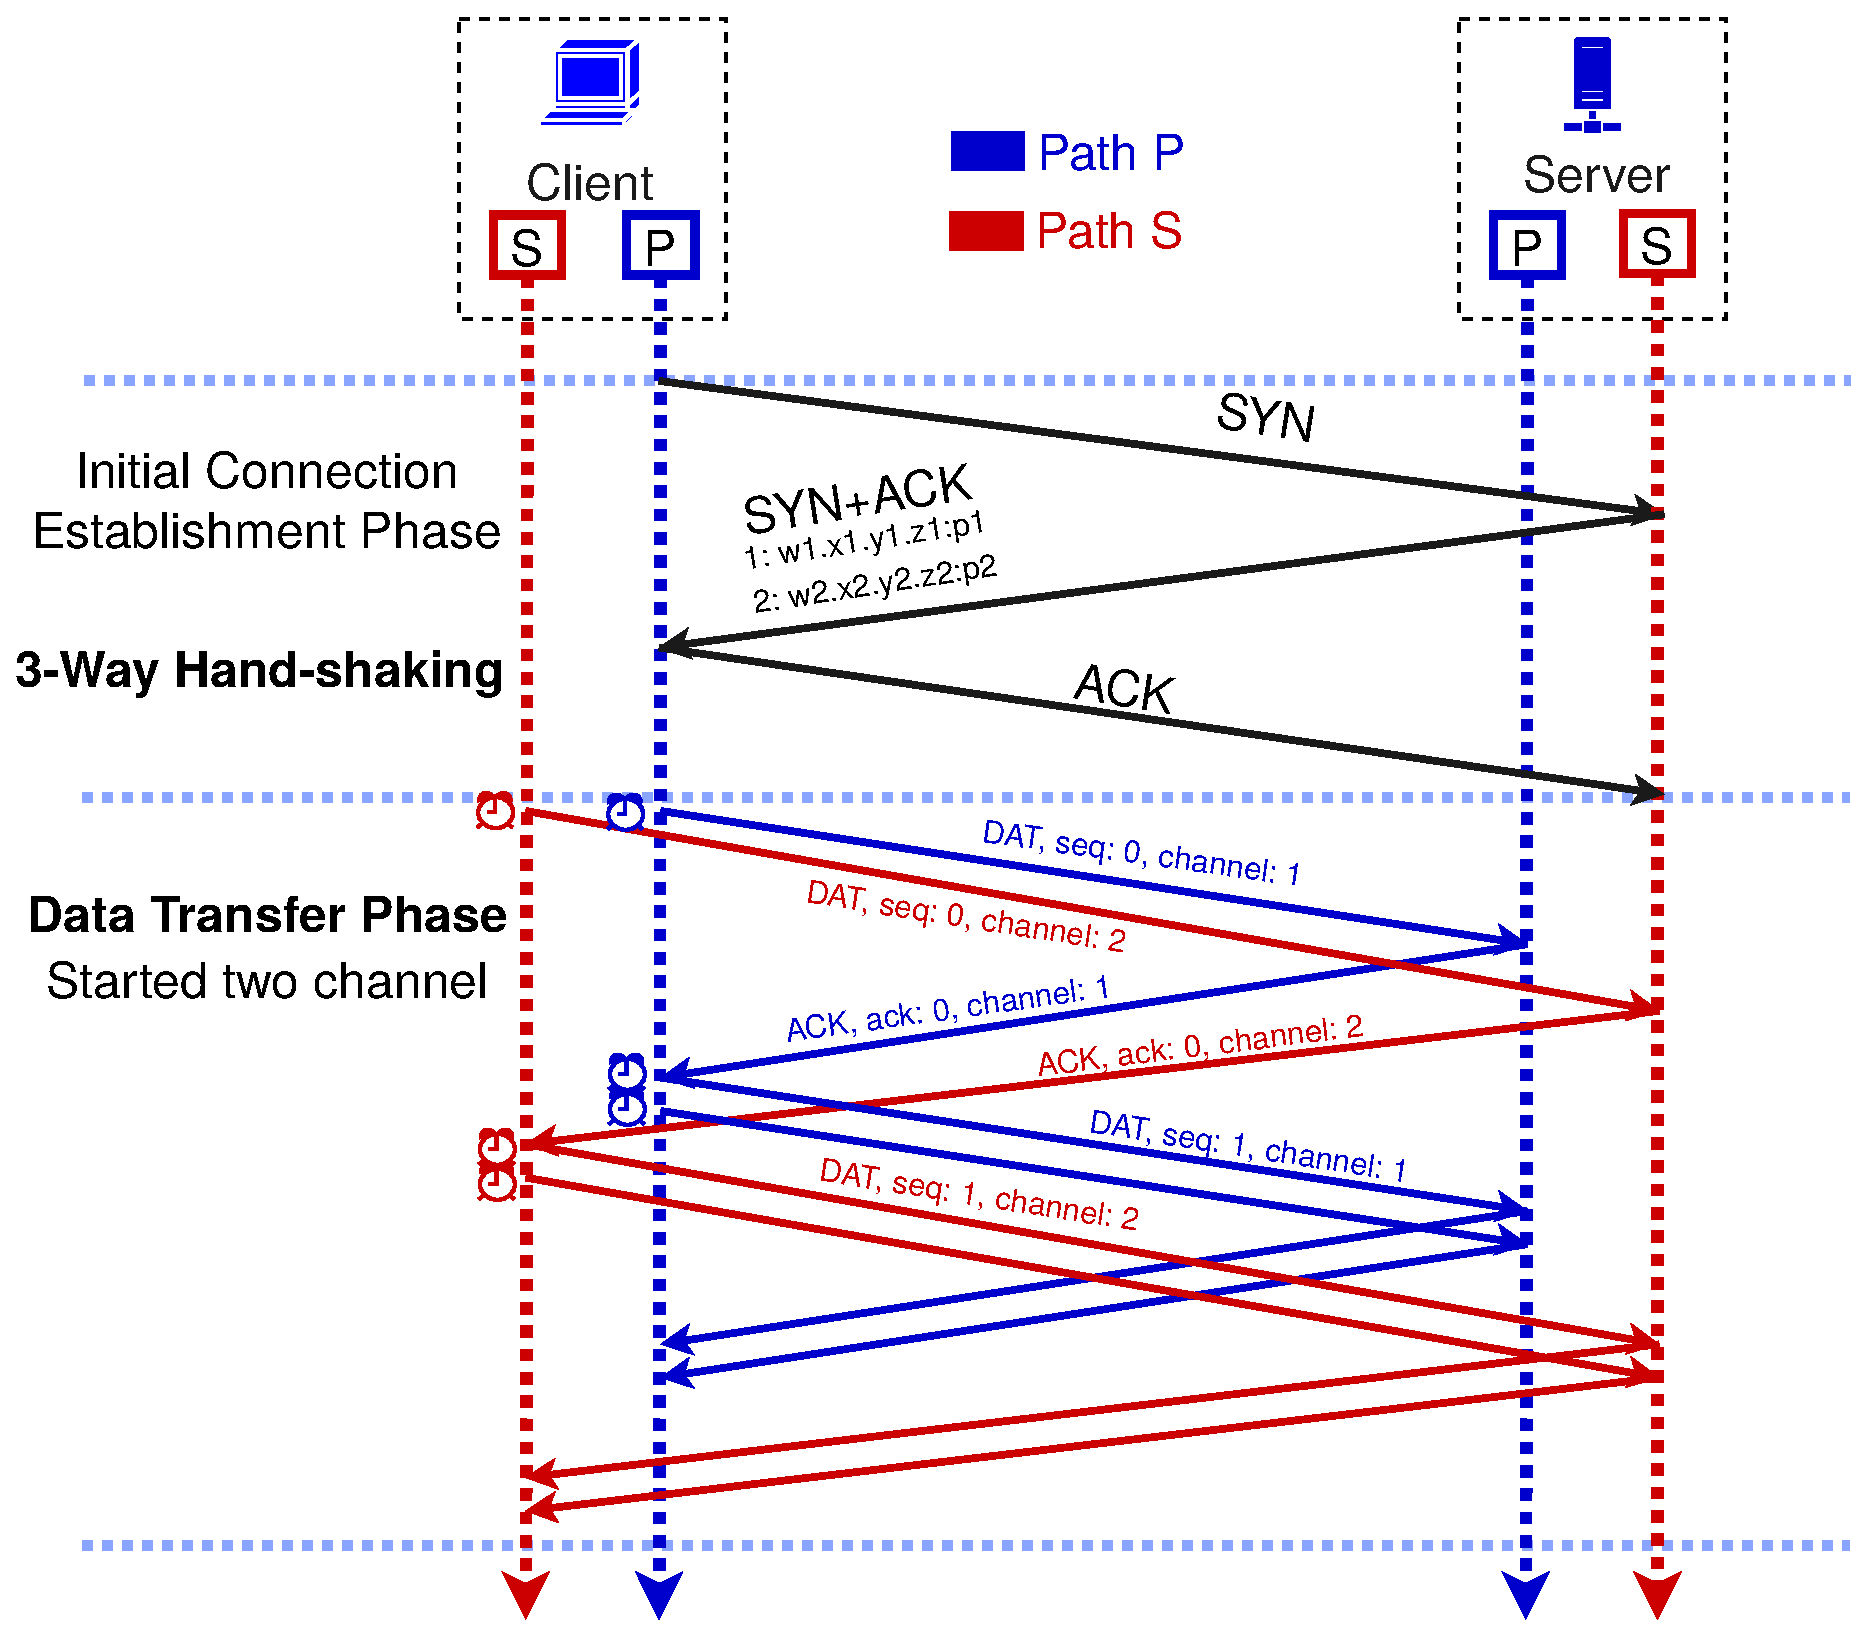
\includegraphics[width=0.8\linewidth]{img/ProtocolDiagram}
%	\caption{Three-way handshaking between client and server and data transfer between them. Handshaking can go between any two pairs of interfaces. Here P is the primary path and S is one of the secondary or alternative paths.}
%	\label{fig:ProtocolDiagram}
%\end{figure}

%Fig.~\ref{fig:ProtocolDiagram} shows the connection establishment and data transmission events for Viscous.
Connection establishment at Viscous follows a three-way handshake procedure similar to the TCP connection establishment. However, as mentioned earlier, Viscous connection establishment is one time and does not depend on the number of flows between the same server, client pair. To establish a connection, a Viscous client sends a synchronization (\texttt{SYN}) packet with a temporary unique identifier or nonce. The nonce or temporary identifier required to identify a client if the \texttt{SYN} packet needs to retransmit. We can use the MAC address of the client as this identifier. On receiving the \texttt{SYN} packet, the Viscous server generates a fingerprint for the client and sends a \texttt{SYN+ACK} packet containing the generated fingerprint. \textit{This fingerprint is used as the connection identifier for the server, client pair}, and every packet between the server and the client includes this fingerprint. In our implementation, we use an SHA256 hash function to generate the fingerprint from the client MAC, server MAC and the current time-stamp used as a unique nonce. It can be noted that different fingerprint is used for different connections, and therefore a fingerprint can uniquely identify a path between a server, client pair. The connection establishment procedure ends with the Viscous client sending an \texttt{ACK} packet. 

During the connection establishment, Viscous server informs all its network addresses to the Viscous client, if the server has multiple interfaces. So, immediately after the connection establishment at one channel, Viscous client initiates all possible channels to Viscous server. There is no requirement to send an extra control packet to complete the channel establishment. After connection establishment, Viscous clients become ready to add flows to the channels, and initiates data transmissions as the applications send data over the flows.

\subsection{Mobility Support in Viscous}
Viscous can support different types of mobility events, as follows.

\subsubsection{Connect-time Mobility}
A connection can fail whenever the server or the client changes its address in between the connection establishment time. With the help of a global name server, this type of mobility can be supported in Viscous. A name server is required to get the new address of the server, when the server changes its IP address. There are two cases that needs to be handled. 
\begin{enumerate}
    \item \textit{Client changes its address just after sending a \texttt{SYN} packet, Server changes its address just after receiving a \texttt{SYN} packet}: This type of failure is automatically recovered by subsequent retries from the client. During the retry, the Viscous client is identified via temporary unique identifier which is used to generate the fingerprint.
    \item \textit{Client or server changes its IP address after receiving the \texttt{SYN+ACK} packet from the server}: As \texttt{SYN+ACK} packet contains the fingerprint, the client can send the \texttt{ACK} packet to complete the three-way handshake by sending the \texttt{ACK} packet to the new server address. The new server address is received with the help from the global name server. However, the success depends on how fast the global name server can update the server IP address against its domain name. If this process fails after three retries, the client re-initiates the connection. 
\end{enumerate}

\subsubsection{Individual Mobility}
Individual mobility event occurs when one of the interfaces from both the devices change its network address. This type of mobility can affect a Viscous connection, only if the affected channel already has some packets under transmission. The subsequent packets will carry the new address to the remote device. This does not create a problem, because the connection is identified by the unique fingerprint between the server and the client. Further, the new IP address can be forwarded via other unaffected channels. If all the channel fails, the affected application can take help from the name-server to find out the new address, and the new channels are creates based on that.

\subsubsection{Simultaneous Mobility}
Simultaneous mobility is rather complex, which occurs when all the interfaces of the server or the client change their network addresses simultaneously. In this scenario, the remote application is not reachable at all. In this event, all existing channels are affected. Therefore, the application needs to get the remote addresses from the name server. Once it get the new addresses, Viscous can continue with the existing connections as the fingerprint remains unchanged.

\subsection{Congestion Control Algorithm}
\label{section:congestion_control}
The congestion control algorithm is the heart of any transport protocol. We design Viscous congestion control algorithm similar to TCP New Reno with SACK option (\cite{RFC2582,RFC2018}). Viscous is designed for short-lived connections. It is expected that application messages are short. So, to reduce overhead, we use fixed size packet. Sequence number used in Viscous are packet based. The congestion control algorithm used in the Viscous have six states {\it Slow Start}, {\it Congestion Avoidance}, {\it Fast Retransmit}, {\it Fast Recovery}, {\it Multi Recovery} and {\it Timeout}. These states are executed in every channel independently. We discuss about these states in details.

\begin{figure}[!h]
	\centering
	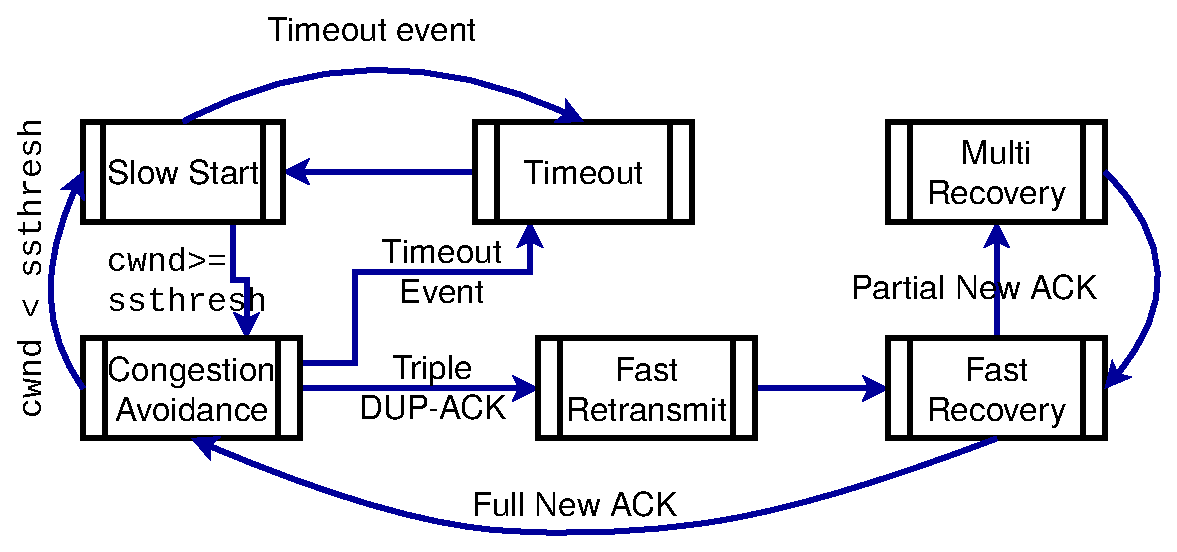
\includegraphics[width=0.8\linewidth]{img/cong_state_tran.eps}
	\caption{State transition diagram in Viscous congestion control algorithm.}
	\label{img:cong-state-tran}
\end{figure}

{\bf Slow Start}: It is similar to TCP (Tahoe, Reno or new-Reno) congestion control. Here, congestion window size ($cwnd$) gets doubled in every round trip time (RTT). To, emulate this effect, we increase $cwnd$ by 1MSS (maximum segment size) upon receiving successful acknowledgment (ACK). The {\it Slow Start} state continue until $cwnd$ reaches Slow Start Threshold ($ssthresh$). Initially $ssthresh$ set to a large value (we use one-forth of the sequence number space {\it i.e.} 16384). 
%So, upon receipent of a successful ACK, $$cwnd_i = cwnd_{i-1} + 1$$

{\bf Congestion Avoidance}: This state is also similar to TCP; in this state, a Viscous channel increases its $cwnd$ by 1MSS in every RTT. Again to emulate this effect, $cwnd$ is updated as $cwnd= cwnd + \frac{1}{cwnd}$ upon receiving successful ACK. The congestion avoidance state continues until the sender receives three duplicate ACKs (triple-DUP ACK) or when timeout event occurs. On triple-DUP ACK event, a Viscous channel immediately goes to {\it Fast Retransmit} and on timeout event, it moves to {\it Timeout} state.

{\bf Fast Retransmit}: In this state, Viscous channel immediately transmits the undelivered packet, and moves to {\it Fast Recovery} state. {\it Fast Retransmit} state is very brief, and it only transmits the missing/undelivered packets. Also, it sets $ssthresh$ to half the current $cwnd$ and mark the maximum sequence number that sent through the channel till now. This marked sequence number will be used in other states.

At this point we need to understand when Viscous sender transmit a packet. Viscous sender transmit a packet when ever there is a packet available in the buffer and $cwnd$ is lesser than flight size. Flight size is the number of packets that have been sent but not acknowledged till now.

{\bf Fast Recovery}: In this state, Viscous channel tries to send a new packet for every DUP-ACKs. When a channel receives a DUP-ACK, it means that the network can deliver further packets as the other end has received some packets. So, sender can transmit some packets. As this DUP-ACK does not decrease the flight size, sender need to increase the $cwnd$ to transmit extra packets. So, we increase $cwnd$ by 1MSS for every DUP-ACKs. It should be noted that, it is not effective increment of $cwnd$. Here we increase $cwnd$ just to send new packet as a response to DUP-ACK. We reset $cwnd$ as soon as {\it Fast Recovery} or {\it Multi Recovery} ends.

In Viscous, we uses a field header called {\tt orig-ack} in its packet. It contains the original packet number, which triggered a DUP-ACK at the receiver side. This field allows a Viscous channel to track the delivered packets at the receiver side like TCP SACK option, and sender don't have to retransmit the acknowledged packet again. During {\it Fast Recovery} state, sender expect to see a new ACK which acknowledges all the the packet it sent till it received last triple DUP-ACKs i.e. the marked sequence number in {\it Fast Retransmission} state. This type of ACK call full new ACK. It means there was only one missing packet. On the other hand, if it receives a new ACK which does not acknowledges all packet upto the mark sequence number, it is partial new ACK. It, means there are multiple packet loss happened the channel. When the sender receives a partial ACK in {\it Fast Recovery} state, channels moves to {\it Multi Recovery} state to recover other missing packets. This behavior is slightly different from TCP SACK option. In SACK option, sender send missing packets  only when retransmission timeout expires. In Viscous, sender can retransmit missing packets as soon as it received partial new ACK if retransmission timeout haven't expired yet.

{\bf Multi Recovery}: In this state, Viscous channel retransmit all the undelivered packets in the sender window. If it exhaust the undelivered packets in the sender window, it again moves to {\it Fast Recovery} state. We use this state to avoid timeouts for multiple packets when there is multiple packet loss in a single window. During this state, $cwnd$ does not change at all.

{\bf Timeout}: It is same as TCP timeout state. Whenever timeout occurs for a packets, Viscous channel moves to {\it Timeout} state. This is also very. In {\it Timeout} state, Viscous channel retransmit the packets and set $ssthresh$ to half of the current $cwnd$ and set $cwnd$ to 1. Immediately after that, Viscous channel moves to {\it SlowStart} state. Timeout event governs by Retransmission Timeout ($rto$) which is calculated as follows.

\begin{equation}
\begin{split}
rttvar &= (1-\beta) * rttvar + \beta * (srtt ~ rtt)\\
srtt &= (1-\alpha)*srtt + \alpha*rtt \\
rto &= srtt + \max(G, 4*rttvar) \\
\end{split}
\end{equation}

where $rtt$ is RTT measured by a single packet and $srtt$ is smoothed RTT. $\alpha$ and $\beta$ are smoothing parameter set to 0.8. $G$ is the granularity of the clock being used in the implementation. This values are similar to the ones set by Jacobson in \cite{Jacobson:1988:CAC:52325.52356,RFC2988}.



